\chapter{State of the Art} \label{chap:sota}

\section*{}

In this chapter is described the state of the art of related work and technologies. It is divided in three parts. Section~\ref{sec:ci} is explained the Continuous Integration process. In section~\ref{sec:ci_tools} is presented the different tools for continuous integration in software development for future contextualization in hardware validation. In section~\ref{sec:hw_val_arc} is presented one hardware validation architecture in which will be based our solution.

\section{Continuous Integration}\label{sec:ci}

Continuous Integration (CI), in Software Engineering, is the process of merging all the working copies of developers to a shared mainline several times a day.
It was first mentioned by Grady Booch in his 1994 book "Object-Oriented Analysis and Design with Applications"~\cite{GradyBooch}, although he did not advocate integrating several times a day. 

Extreme programming (XP) adopted this concept, when Kent Beck described XP~\cite{KentBeck} as an agile methodology designed for improving productivity, flexibility and teamwork in projects, and did advocate integrating more than once per day, not leaving "unintegrated" code for more than a couple of hours, thus presenting CI as one of its practices.

CI was set to resolve prevent integration problems, referred to "Integration Hell" in early characterizations of XP, where developers used to divide work in modules, that once completed, would be integrated to create the application as a whole. It was a costly process in terms of time and effort, arising a number of bugs in the process.

The idea behind CI is to reduce this issues by integrating early and often, so as to avoid the "integration hell".

\subsection{Process}

Continuous Integration is a cyclic process, as seen in the figure \ref{fig:ci_process}, divided in the following steps:

\begin{enumerate}
\item \textbf{Commit -} Developer modifies the code, tests it and commits to the repository;
\item \textbf{Build -} Code is fetched from the repository, integrated and built;
\item \textbf{Test -} Tests are performed on the build, followed by a report of the outcome;
\item \textbf{Report -} Developers are notified about the build and tests results\\
\end{enumerate}

  \begin{figure}[H]
  \centering
      \makebox[\textwidth][c]{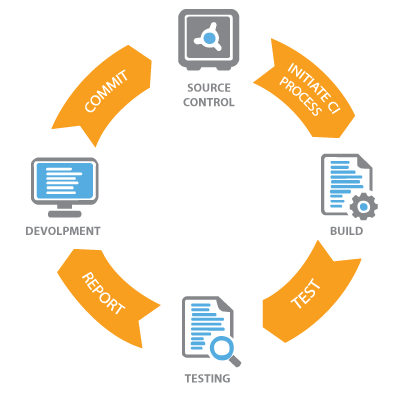
\includegraphics[width=0.5\textwidth]{ci_process}}
      \caption{Continuous Integration Process}
      \label{fig:ci_process}
  \end{figure}

The process is dependent of the build and tests duration. It is expected to be fast so it can be run several times a day.

\subsection{Components}\label{sc:ciComponents}
In this section are enumerated each component in the CI process.

\subsubsection{Developers}
Code developers are responsible for the creation of software. Continuous Integration is backed by several important principles and practices~\cite{CIimproveSQRR}:  

\begin{itemize}
\item \textbf{Check in frequently} - Frequent commits means that smaller amount of code changed, which leads to an easier process of finding bugs;
\item \textbf{Create automated tests} - Tests should be automated and have high code coverage;
\item \textbf{Don’t check in broken code} - Before commit, developers should test the code locally so errors aren't unnecessary introduced;  
\item \textbf{Don’t check in when the build is broken} - If a build is broken, it should be made top priority an effort in fixing it, so the errors do not propagate.
\end{itemize}

Many teams develop rituals around these policies, meaning the teams effectively manage themselves, knowing that if software is broken, they will receive immediate feedback.

\subsubsection{Repository}\label{repository}
A central repository with the project code using a Source Code Management (SCM) tool or Version Control System (VCS) is needed to perform a successful CI, maintaining the code reachable so the developers can get the most recent version of the source code.
This systems are important for software development as they serve as backup for programmers. It is possible to revert changes or pull previous code, allowing its use without the risk of breaking working code.
Repositories should contain the source code and everything else needed to create a build, such as: test files and scripts, database schemas, libraries and install scripts. Everything needed to run the software in a new machine.

\subsubsection{CI Server}
The CI server is the instrument behind Continuous Integration. It is used to implement continuous process of applying quality control of the software, by pulling the latest code from the repository, create a build and report the developers a feedback of the outcome.
There are several CI tools implementing this system, which we will talk in section \ref{sec:ci_tools} with more detail.

\subsection{Value}
By adopting Continuous Integration, you not only reduce risks and catch bugs quickly, but also move rapidly to working software.

With low-risk releases, you can quickly adapt to business requirements and user needs. This allows for greater collaboration between ops and delivery, fueling real change in your organization, and turning your release process into a business advantage.

\section{Continuous Integration Tools}\label{sec:ci_tools}

In order to set up a successful agile software development environment, it is essential to include a method of continuous integration in the process~\cite{Abdul2012}. This practice can be easily adapted to the hardware validation process, since it operates the same way as in software development:
\begin{enumerate}
\item Hardware logic is modified;
\item Firmware is built and deployed on the physical hardware;
\item Automated tests are run;
\item Hardware is validated.\\
\end{enumerate}

To contextualize this process into the hardware validation process, we must first choose a continuous integration tool before designing the architecture of the system.
It is known that there is a wide range of choices for continuous integration tools available, but for this project it was selected Jenkins as the preferred one. 

\subsection{Jenkins CI}\label{jenkins}

Jenkins~\cite{kn:Jenkins} is a continuous integration and continuous delivery tool application, used to build and test software projects and help developers integrate new changes and features to the project. It also provides ways to delineate customized build pipelines and integrate with several testing and deployment technologies.

It is the application of choice to create our system thanks to the several features it offers, such as:

\begin{itemize}
\item \textbf{Open Source} - Jenkins can be extended and modified in its majority, and makes uncomplicated to develop new plugins. This allows the creation of the dashboard plugin proposed;
\item \textbf{Automated Jobs / Jobs Management} - Jenkins can integrate with most software configuration management and build tools available. With this it is possible an easy script management of jobs to build, deploy and test the firmware developed;
\item \textbf{Build Reports} - The tool can automatically receive and generate logs of successful or failed builds, which can then be parsed (for example into an XML) and eventually used in a plugin or external application;
\item \textbf{Distributed System} - Jenkins can distribute builds and test loads to specific machines with the requested configurations.
\end{itemize}

\subsubsection{Jenkins Pipeline Jobs}\label{jenkinsPipeline}

In modern environment, delivering innovative ideas in a fast and reliable manner is extremely significant for any organization to better respond the dynamic market requirements \cite{Soni2015}. 

Recently, inside the Jenkins tool, was created a new ecosystem that allows implementing jobs in a domain specific language. It is referred to as Pipeline~\citet{jnks:pipeline} (formerly known as Workflow).

Pipeline is a powerful tool available for Jenkins users to implement various software delivery pipelines in code.

Since any peripheral hardware device can be attached to a Jenkins node, and these nodes requiring Java only, almost every development machine can be attached. A Sample scheme can be seen in the  figure~\ref{fig:connectionScheme}.

  \begin{figure}[H]
  \centering
      \makebox[\textwidth][c]{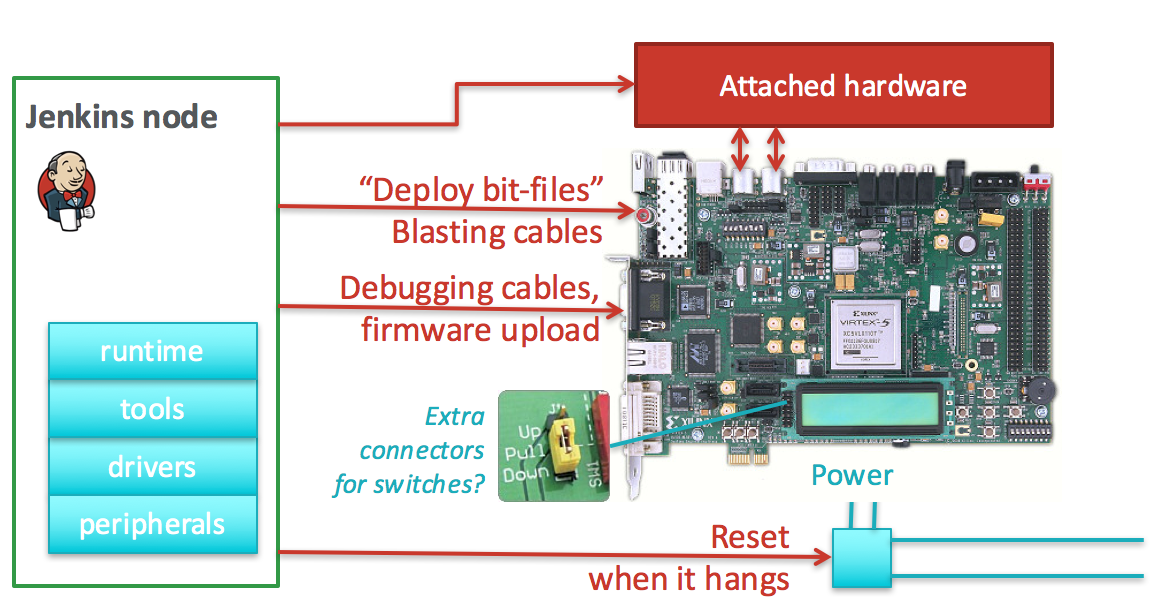
\includegraphics[width=1\textwidth]{connectBoard}}
      \caption{Common connection scheme ~\cite{jnks:automatedPipeline}}
      \label{fig:connectionScheme}
  \end{figure}
  
When connected, Jenkins jobs could invoke common EDA tools via command-line interfaces, which can be easily done by a Execute shell build steps in free-style projects.

Pipeline as Code is an approach for describing complex automation flows in software lifecycles, e.g: build, delivery, deployment.

In Jenkins there are two most popular plugins: Pipeline~\citet{jnks:pipeline} and Job DSL~\cite{jnks:dsl}. JobDSL Plugin internally generates common freestyle jobs according to the script, so it’s functionality is similar to the classic approaches. Pipeline is fundamentally different, because it provides a new engine controlling flows independently from particular nodes and workspaces. So it provides a higher job description level, which was not available in Jenkins before.

Accordingly to Oleg Nenashev~\cite{jnks:automatedPipeline}, there are several Pipeline features that may be of value to embedded and hardware projects.

\begin{itemize}
\item Robustness against restarts of Jenkins master.
\item Robustness against network disconnects. sh() steps are based on the Durable Task plugin~\cite{jnks:durableTask}, so Jenkins can safely continue the execution flow once the node reconnects to the master.
\item Possibility to run tasks on multiple nodes without creating complex flows based on job triggers and copy artifact steps. Achieved via combination of parallel() and node() steps.
\item Ability to store the shared logic in standalone Pipeline libraries
\end{itemize}

In conclusion, Jenkins is a powerful automation framework that can be used in many areas. Although it has no dedicated plugins for test runs on hardware, it provides diverse general-purpose "building blocks", that allow the implementation of any flow.

Pipeline as code can greatly simplify these complex implementations in Jenkins. It continues to evolve and extend support of use-cases.

\section{Hardware Validation Architectures}\label{sec:hw_val_arc}

Subsequently to deciding the CI tool to use, we must start designing the architecture of the target environment. The framework we came across that accomplishes our goal to some extent was the LAVA project.

\subsection{LAVA}\label{lava}

The Linaro Automated Validation Architecture (LAVA) project~\cite{kn:LAVA} is a "continuous integration system for deploying operating systems onto physical and virtual hardware for running tests". It can run simple boot loading and system level tests, where the results can be exported and inspected subsequently.

It is composed by two main components, as seen in the figure~\ref{fig:lava}: 

\begin{itemize}
\item The LAVA Server: a web application that provides a central scheduler, dashboard for job monitoring and test result visualization;
\item The LAVA Dispatcher: a sub-system that manages communication to the physical test devices.
\end{itemize}

The overall idea is allowing us to make continuous testing, quality control and automatic validation for projects of all sizes.

%Careful with this
\clearpage

\begin{figure}[H]
\centering
\makebox[\textwidth][c]{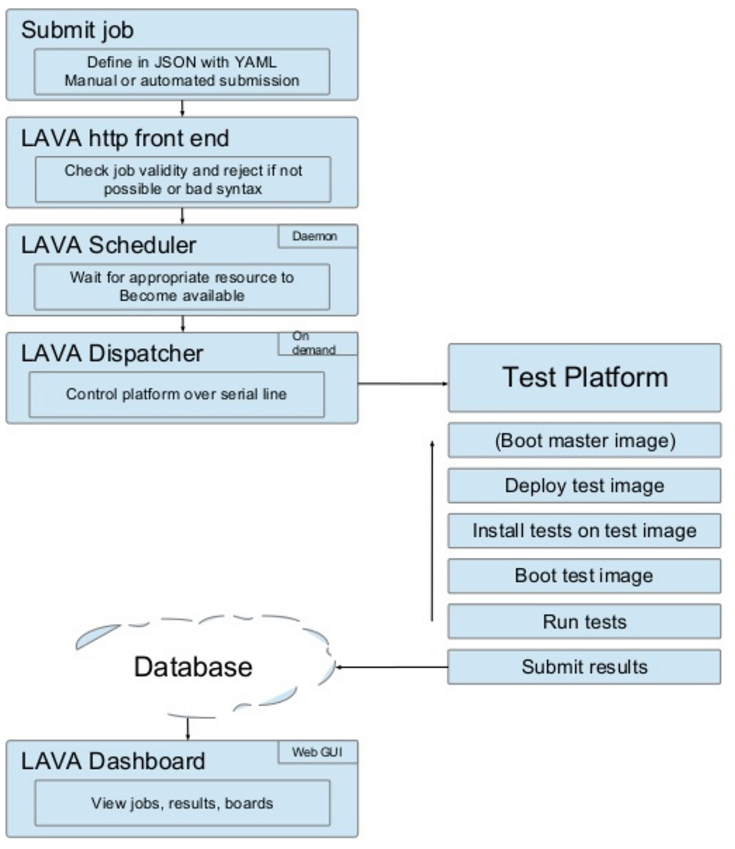
\includegraphics[width=1\textwidth]{lava_workflow}}
\caption{LAVA Workflow}
\label{fig:lava}
\end{figure}

It is to note that LAVA itself doesn't run the tests, it is only an enabler as it does not define what can be run. It is a merely black-box to CI, since the test jobs still have to be provided by an external source (usually Jenkins).\\
The framework serves to test the boards from the Linaro validation lab in Cambridge, where all devices have the same LAVA interface.

%https://www.youtube.com/watch?v=hS382L6EYrE
%http://www.slideshare.net/linaroorg/01-lava-introductionandupdatesdavemilo1

\section{Conclusions}
The market is full of CI tools available to use, but it is not very explored in the hardware validation context.

Since Synopsys already started to implement a Continuous Integration environment using Jenkins, with automated jobs by this time created in the application, and it providing key features for the goal system, makes sense to continue this approach to develop a new plugin for the tool.

Concluding, we can adapt the LAVA architecture to Synopsys interfaces using Jenkins, by using the job management and distributed system features as the central scheduler and dispatcher, and creating the dashboard plugin to supervise the test results.
